\chapter{Docker registry}

The Registry is a stateless, highly scalable server side application that stores and lets you distribute Docker images. \cite{docker-registry}

The Registry is the only reasonable way how to distribute Docker images inside a network. When a developer creates new image with his application, there are 2 ways how to get it to production. The first one is to do it through a Dockerfile. The second one is using Docker image. In the future it would be nice to have a whole system, where you only put a new Dockerfile (let’s say simply by merging your dev branch with the new Dockerfile to the master branch in Git) and the system will then build your image, tag it properly and upload it to the Docker registry. This is a state we want to achieve eventually, but it currently takes more work than we can afford to build a system like this.

So the second way is that Deznam.cz will have to create a Docker registry, where developers can push their images and then send tickets to administrator to get them in production. So I have to study the Docker registry more deeply. The Registry is an application that you can run on server. Then every developer have to tag his image with server name and port on which the registry is running and append his own name. In Seznam.cz we are prefixing each name of application with the department name and the ``szn" prefix. For example \lstinline{szn-fulltext-APP_NAME}. So basically now each developer will have to tag his image similarly like that: \lstinline{REGISTRY_URL /fulltext/APP_NAME} and push it. The Registry URL has to be easy to remember and we need to be sure it does not cause conflict in the future. You also have to define which images will be included in the Kubernetes pod and those pod definitions have to be created in a cooperation of developers with administrators. And if there are different names for the registry in development, staging and production environment those pod definitions will have to be updated each time which might easily lead to mistakes.

We have to create development, staging and production Docker registry servers where images will be stored. The development registry can be a standard server with a large disk space because many versions of images will be stored here. Developers will have unlimited access to it via the Docker command line tool and no special policy will be defined here.

We cannot have the dev registry with authentication because when pushing new image to registry you would have to set password. As the credentials are stored in \lstinline{\$HOME/.dockercfg} and every developer in our development environment has root privileges, such practice would be insecure and untrusty.

After successfully creating an image and uploading to the dev server, the developer will have to send a request to an administrator to deploy it. In Seznam.cz we have a custom request tracker and when someone want to deploy something, we have to send a RT ticket with a number of the particular Debian package version. The only difference with Docker would be that the developer will  send an image signature hash created by Docker. This way there will always be a possibility to authenticate possible and the developer who sent the ticket will be responsible for his image.

The administrator will then pull the image from the dev registry and push it to the staging registry and then to the production registry.

When Kubernetes starts a new pod, the Kubernetes master node downloads the image from registry (if it’s not present already) and run it. This logic makes the registry server a bottleneck for the entire cluster. When the master node cannot pull from the registry server, the application won’t start. And even when app is running, if the registry server fails and then Kubernetes decides to migrate this pod from one server to another because of load balancing or something else, application can easily become unavailable. That means that Seznam.cz’s Docker registry in the production environment has to run on high availability servers.

The Docker registry is an application which provides an API for clients and the storage itself is delegated to drivers. The default driver is posix filesystem.  As is said in the manual, this default driver is fine for small deployments and in our conditions will be fine for development environment where physical hard drivers will be mirrored. Development registry server does not have to be high availability and there is always a way how to start custom registry even on local machine.

The Docker registry storage drivers provided are \cite{docker-registry-storages}:

\begin{itemize}
  \item \textbf{inmemory}: A temporary storage driver using a local inmemory map. This exists solely for reference and testing.
  \item \textbf{filesystem}: A local storage driver configured to use a directory tree in the local filesystem.
  \item \textbf{s3}: A driver storing objects in an Amazon Simple Storage Solution (S3) bucket.
  \item \textbf{azure}: A driver storing objects in Microsoft Azure Blob Storage.
  \item \textbf{rados}: A driver storing objects in a Ceph Object Storage pool.
  \item \textbf{swift}: A driver storing objects in Openstack Swift.
  \item \textbf{oss}: A driver storing objects in Aliyun OSS.
  \item \textbf{gcs}: A driver storing objects in a Google Cloud Storage bucket.
\end{itemize}


From all these drivers provided the only two options we can use are rados, with Ceph Object Storage and swift with Openstack Swift storage. And because in Seznam.cz there are administrators who are well acquainted with the technology of Swift, we decided that for the production registry we will use swift as a storage driver.

So the final model is shown in the following figure \ref{fig:seznam-docker-registry}.
                
\begin{figure}[htb]\centering
  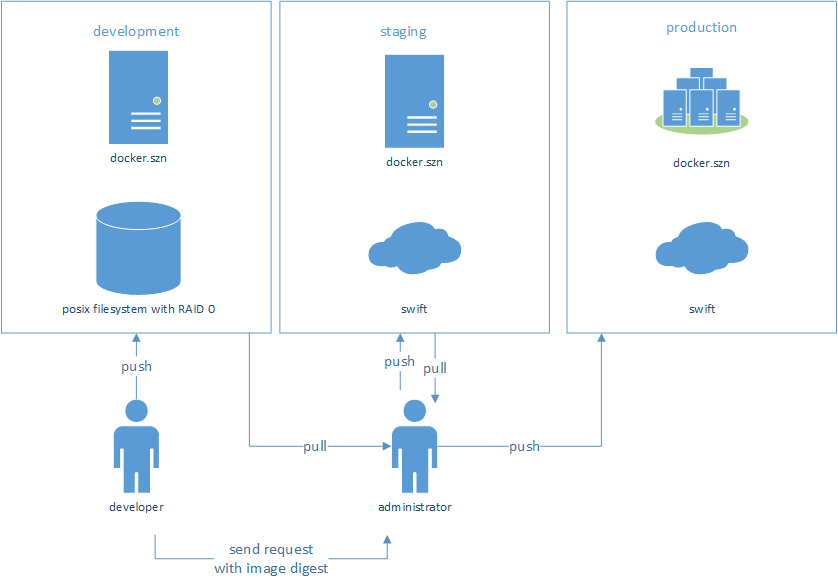
\includegraphics[width=1\textwidth]{images/registry.png}
  \caption
    {Seznam.cz Docker registry architecture}
  \label{fig:seznam-docker-registry}
\end{figure}
